% Options for packages loaded elsewhere
\PassOptionsToPackage{unicode}{hyperref}
\PassOptionsToPackage{hyphens}{url}
%
\documentclass[
]{article}
\usepackage{lmodern}
\usepackage{amssymb,amsmath}
\usepackage{ifxetex,ifluatex}
\ifnum 0\ifxetex 1\fi\ifluatex 1\fi=0 % if pdftex
  \usepackage[T1]{fontenc}
  \usepackage[utf8]{inputenc}
  \usepackage{textcomp} % provide euro and other symbols
\else % if luatex or xetex
  \usepackage{unicode-math}
  \defaultfontfeatures{Scale=MatchLowercase}
  \defaultfontfeatures[\rmfamily]{Ligatures=TeX,Scale=1}
\fi
% Use upquote if available, for straight quotes in verbatim environments
\IfFileExists{upquote.sty}{\usepackage{upquote}}{}
\IfFileExists{microtype.sty}{% use microtype if available
  \usepackage[]{microtype}
  \UseMicrotypeSet[protrusion]{basicmath} % disable protrusion for tt fonts
}{}
\makeatletter
\@ifundefined{KOMAClassName}{% if non-KOMA class
  \IfFileExists{parskip.sty}{%
    \usepackage{parskip}
  }{% else
    \setlength{\parindent}{0pt}
    \setlength{\parskip}{6pt plus 2pt minus 1pt}}
}{% if KOMA class
  \KOMAoptions{parskip=half}}
\makeatother
\usepackage{xcolor}
\IfFileExists{xurl.sty}{\usepackage{xurl}}{} % add URL line breaks if available
\IfFileExists{bookmark.sty}{\usepackage{bookmark}}{\usepackage{hyperref}}
\hypersetup{
  pdftitle={Reproducible Research: Peer Assessment 1},
  hidelinks,
  pdfcreator={LaTeX via pandoc}}
\urlstyle{same} % disable monospaced font for URLs
\usepackage[margin=1in]{geometry}
\usepackage{color}
\usepackage{fancyvrb}
\newcommand{\VerbBar}{|}
\newcommand{\VERB}{\Verb[commandchars=\\\{\}]}
\DefineVerbatimEnvironment{Highlighting}{Verbatim}{commandchars=\\\{\}}
% Add ',fontsize=\small' for more characters per line
\usepackage{framed}
\definecolor{shadecolor}{RGB}{248,248,248}
\newenvironment{Shaded}{\begin{snugshade}}{\end{snugshade}}
\newcommand{\AlertTok}[1]{\textcolor[rgb]{0.94,0.16,0.16}{#1}}
\newcommand{\AnnotationTok}[1]{\textcolor[rgb]{0.56,0.35,0.01}{\textbf{\textit{#1}}}}
\newcommand{\AttributeTok}[1]{\textcolor[rgb]{0.77,0.63,0.00}{#1}}
\newcommand{\BaseNTok}[1]{\textcolor[rgb]{0.00,0.00,0.81}{#1}}
\newcommand{\BuiltInTok}[1]{#1}
\newcommand{\CharTok}[1]{\textcolor[rgb]{0.31,0.60,0.02}{#1}}
\newcommand{\CommentTok}[1]{\textcolor[rgb]{0.56,0.35,0.01}{\textit{#1}}}
\newcommand{\CommentVarTok}[1]{\textcolor[rgb]{0.56,0.35,0.01}{\textbf{\textit{#1}}}}
\newcommand{\ConstantTok}[1]{\textcolor[rgb]{0.00,0.00,0.00}{#1}}
\newcommand{\ControlFlowTok}[1]{\textcolor[rgb]{0.13,0.29,0.53}{\textbf{#1}}}
\newcommand{\DataTypeTok}[1]{\textcolor[rgb]{0.13,0.29,0.53}{#1}}
\newcommand{\DecValTok}[1]{\textcolor[rgb]{0.00,0.00,0.81}{#1}}
\newcommand{\DocumentationTok}[1]{\textcolor[rgb]{0.56,0.35,0.01}{\textbf{\textit{#1}}}}
\newcommand{\ErrorTok}[1]{\textcolor[rgb]{0.64,0.00,0.00}{\textbf{#1}}}
\newcommand{\ExtensionTok}[1]{#1}
\newcommand{\FloatTok}[1]{\textcolor[rgb]{0.00,0.00,0.81}{#1}}
\newcommand{\FunctionTok}[1]{\textcolor[rgb]{0.00,0.00,0.00}{#1}}
\newcommand{\ImportTok}[1]{#1}
\newcommand{\InformationTok}[1]{\textcolor[rgb]{0.56,0.35,0.01}{\textbf{\textit{#1}}}}
\newcommand{\KeywordTok}[1]{\textcolor[rgb]{0.13,0.29,0.53}{\textbf{#1}}}
\newcommand{\NormalTok}[1]{#1}
\newcommand{\OperatorTok}[1]{\textcolor[rgb]{0.81,0.36,0.00}{\textbf{#1}}}
\newcommand{\OtherTok}[1]{\textcolor[rgb]{0.56,0.35,0.01}{#1}}
\newcommand{\PreprocessorTok}[1]{\textcolor[rgb]{0.56,0.35,0.01}{\textit{#1}}}
\newcommand{\RegionMarkerTok}[1]{#1}
\newcommand{\SpecialCharTok}[1]{\textcolor[rgb]{0.00,0.00,0.00}{#1}}
\newcommand{\SpecialStringTok}[1]{\textcolor[rgb]{0.31,0.60,0.02}{#1}}
\newcommand{\StringTok}[1]{\textcolor[rgb]{0.31,0.60,0.02}{#1}}
\newcommand{\VariableTok}[1]{\textcolor[rgb]{0.00,0.00,0.00}{#1}}
\newcommand{\VerbatimStringTok}[1]{\textcolor[rgb]{0.31,0.60,0.02}{#1}}
\newcommand{\WarningTok}[1]{\textcolor[rgb]{0.56,0.35,0.01}{\textbf{\textit{#1}}}}
\usepackage{graphicx,grffile}
\makeatletter
\def\maxwidth{\ifdim\Gin@nat@width>\linewidth\linewidth\else\Gin@nat@width\fi}
\def\maxheight{\ifdim\Gin@nat@height>\textheight\textheight\else\Gin@nat@height\fi}
\makeatother
% Scale images if necessary, so that they will not overflow the page
% margins by default, and it is still possible to overwrite the defaults
% using explicit options in \includegraphics[width, height, ...]{}
\setkeys{Gin}{width=\maxwidth,height=\maxheight,keepaspectratio}
% Set default figure placement to htbp
\makeatletter
\def\fps@figure{htbp}
\makeatother
\setlength{\emergencystretch}{3em} % prevent overfull lines
\providecommand{\tightlist}{%
  \setlength{\itemsep}{0pt}\setlength{\parskip}{0pt}}
\setcounter{secnumdepth}{-\maxdimen} % remove section numbering

\title{Reproducible Research: Peer Assessment 1}
\author{}
\date{\vspace{-2.5em}}

\begin{document}
\maketitle

\hypertarget{loading-libraries}{%
\subsection{Loading libraries}\label{loading-libraries}}

The first step is to load all the necessary libraries to run the code

\begin{Shaded}
\begin{Highlighting}[]
\KeywordTok{library}\NormalTok{(dplyr)}
\KeywordTok{library}\NormalTok{(stringr)}
\KeywordTok{library}\NormalTok{(reshape2)}
\KeywordTok{library}\NormalTok{(chron)}
\KeywordTok{library}\NormalTok{(data.table)}
\KeywordTok{library}\NormalTok{(ggplot2)}
\KeywordTok{library}\NormalTok{(grid)}
\KeywordTok{library}\NormalTok{(gridExtra)}
\KeywordTok{library}\NormalTok{(lattice)}
\KeywordTok{library}\NormalTok{()}
\end{Highlighting}
\end{Shaded}

\hypertarget{loading-and-preprocessing-the-data}{%
\subsection{Loading and preprocessing the
data}\label{loading-and-preprocessing-the-data}}

The next step is to load and process the data. For this purposes, we
first download the file and save it to the working directory:

\begin{Shaded}
\begin{Highlighting}[]
\NormalTok{dirPath <-}\StringTok{ }\KeywordTok{getwd}\NormalTok{()}
\KeywordTok{download.file}\NormalTok{(}\StringTok{'https://d396qusza40orc.cloudfront.net/repdata%2Fdata%2Factivity.zip'}\NormalTok{, }
              \DataTypeTok{destfile =} \KeywordTok{paste}\NormalTok{(dirPath,}\StringTok{'/activity.zip'}\NormalTok{, }\DataTypeTok{sep =} \StringTok{''}\NormalTok{))}
\end{Highlighting}
\end{Shaded}

Second, we unzip the file to the same working directory and read it to a
data table:

\begin{Shaded}
\begin{Highlighting}[]
\KeywordTok{unzip}\NormalTok{(}\DataTypeTok{zipfile =} \StringTok{'activity.zip'}\NormalTok{, }\DataTypeTok{exdir =} \KeywordTok{getwd}\NormalTok{())}
\NormalTok{activity_dt <-}\StringTok{ }\KeywordTok{read.table}\NormalTok{(}\DataTypeTok{file =} \StringTok{'activity.csv'}\NormalTok{, }\DataTypeTok{header =} \OtherTok{TRUE}\NormalTok{, }\DataTypeTok{sep =} \StringTok{','}\NormalTok{)}
\end{Highlighting}
\end{Shaded}

And finally, before starting to plot and answer the assignment
questions, we need to do some data preparations - validate Data formats
and make a data table with NAs removed:

\begin{verbatim}
activity_dt$date <- as.Date(activity_dt$date, origin = '2012-10-01')
activity_dt_NM <- na.omit(activity_dt)
\end{verbatim}

\hypertarget{what-is-mean-total-number-of-steps-taken-per-day}{%
\subsection{What is mean total number of steps taken per
day?}\label{what-is-mean-total-number-of-steps-taken-per-day}}

To answer this question, we need to do some calculations first.

\begin{enumerate}
\def\labelenumi{\arabic{enumi}.}
\tightlist
\item
  Calculating steps by day:
\end{enumerate}

\begin{verbatim}
steps_ByDay <- aggregate(activity_dt$steps, by = list(activity_dt$date), sum)
colnames(steps_ByDay) <- c('Days', 'Total_steps')
\end{verbatim}

\begin{enumerate}
\def\labelenumi{\arabic{enumi}.}
\setcounter{enumi}{1}
\tightlist
\item
  Calculating the mean and the median:
\end{enumerate}

\begin{Shaded}
\begin{Highlighting}[]
\NormalTok{steps_mean <-}\StringTok{ }\KeywordTok{round}\NormalTok{(}\KeywordTok{mean}\NormalTok{(steps_ByDay}\OperatorTok{$}\NormalTok{Total_steps, }\DataTypeTok{na.rm =} \OtherTok{TRUE}\NormalTok{), }\DataTypeTok{digits =} \DecValTok{4}\NormalTok{) }
\NormalTok{steps_median <-}\StringTok{ }\KeywordTok{round}\NormalTok{(}\KeywordTok{median}\NormalTok{(steps_ByDay}\OperatorTok{$}\NormalTok{Total_steps, }\DataTypeTok{na.rm =} \OtherTok{TRUE}\NormalTok{), }\DataTypeTok{digits =} \DecValTok{4}\NormalTok{)}
\end{Highlighting}
\end{Shaded}

\begin{enumerate}
\def\labelenumi{\arabic{enumi}.}
\setcounter{enumi}{2}
\tightlist
\item
  And finally, plotting and reporting both the data, the mean and the
  median:
\end{enumerate}

\begin{Shaded}
\begin{Highlighting}[]
\CommentTok{#plotting histogram}
\KeywordTok{ggplot}\NormalTok{(}\DataTypeTok{data =}\NormalTok{ steps_ByDay, }\KeywordTok{aes}\NormalTok{(}\DataTypeTok{x=}\NormalTok{Days, }\DataTypeTok{y =}\NormalTok{ Total_steps)) }\OperatorTok{+}
\StringTok{      }\KeywordTok{geom_histogram}\NormalTok{(}\DataTypeTok{stat =} \StringTok{'identity'}\NormalTok{, }\KeywordTok{aes}\NormalTok{(}\DataTypeTok{fill =}\NormalTok{ Total_steps)) }\OperatorTok{+}
\CommentTok{#adding mean & median geoms}
\StringTok{      }\KeywordTok{geom_hline}\NormalTok{(}\KeywordTok{aes}\NormalTok{(}\DataTypeTok{yintercept =}\NormalTok{ steps_mean, }\DataTypeTok{color =} \KeywordTok{paste}\NormalTok{(}\StringTok{'Mean: '}\NormalTok{, steps_mean)), }
                 \DataTypeTok{linetype =} \DecValTok{2}\NormalTok{, }\DataTypeTok{size =} \DecValTok{1}\NormalTok{) }\OperatorTok{+}
\StringTok{      }\KeywordTok{geom_hline}\NormalTok{(}\KeywordTok{aes}\NormalTok{(}\DataTypeTok{yintercept =}\NormalTok{ steps_median, }\DataTypeTok{color =} \KeywordTok{paste}\NormalTok{(}\StringTok{'Median: '}\NormalTok{, steps_median)), }
                 \DataTypeTok{linetype =} \DecValTok{2}\NormalTok{, }\DataTypeTok{size =} \DecValTok{1}\NormalTok{) }\OperatorTok{+}
\StringTok{      }\KeywordTok{scale_color_manual}\NormalTok{(}\StringTok{'Mean & Median'}\NormalTok{, }\DataTypeTok{values =} \KeywordTok{c}\NormalTok{(}\DecValTok{1}\NormalTok{, }\DecValTok{2}\NormalTok{))}
\end{Highlighting}
\end{Shaded}

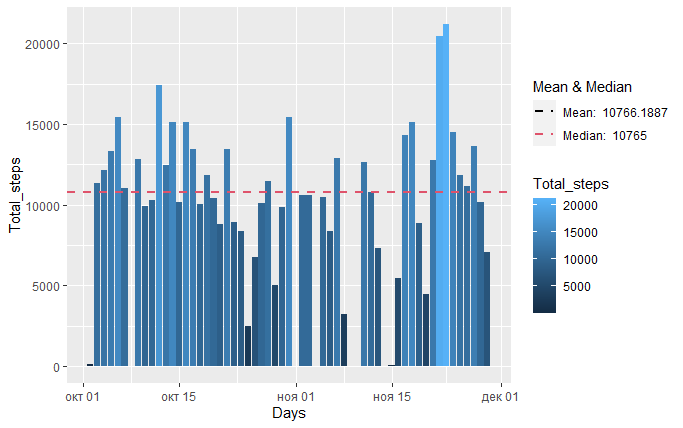
\includegraphics[width=1\linewidth]{./Rplot_1}

\hypertarget{what-is-the-average-daily-activity-pattern}{%
\subsection{What is the average daily activity
pattern?}\label{what-is-the-average-daily-activity-pattern}}

To answer this question, we need to do some calculations first.

\begin{enumerate}
\def\labelenumi{\arabic{enumi}.}
\tightlist
\item
  Calculating average steps by interval:
\end{enumerate}

\begin{Shaded}
\begin{Highlighting}[]
\NormalTok{steps_ByInterval <-}\StringTok{ }\KeywordTok{aggregate}\NormalTok{(activity_dt_NM}\OperatorTok{$}\NormalTok{steps, }\DataTypeTok{by =} \KeywordTok{list}\NormalTok{(activity_dt_NM}\OperatorTok{$}\NormalTok{interval), mean)}
\KeywordTok{colnames}\NormalTok{(steps_ByInterval) <-}\StringTok{ }\KeywordTok{c}\NormalTok{(}\StringTok{'Interval'}\NormalTok{, }\StringTok{'Avg_steps'}\NormalTok{)}
\end{Highlighting}
\end{Shaded}

\begin{enumerate}
\def\labelenumi{\arabic{enumi}.}
\setcounter{enumi}{1}
\tightlist
\item
  Calculating maximum steps and the corresponding interval:
\end{enumerate}

\begin{Shaded}
\begin{Highlighting}[]
\NormalTok{max_AvgSteps <-}\StringTok{ }\KeywordTok{max}\NormalTok{(steps_ByInterval}\OperatorTok{$}\NormalTok{Avg_steps)}
\NormalTok{max_interval <-}\StringTok{ }\KeywordTok{with}\NormalTok{(steps_ByInterval, Interval[Avg_steps }\OperatorTok{==}\StringTok{ }\NormalTok{max_AvgSteps])}
\end{Highlighting}
\end{Shaded}

\begin{enumerate}
\def\labelenumi{\arabic{enumi}.}
\setcounter{enumi}{2}
\tightlist
\item
  Last step, plotting the data along with maximum values:
\end{enumerate}

\begin{Shaded}
\begin{Highlighting}[]
\KeywordTok{plot}\NormalTok{(steps_ByInterval}\OperatorTok{$}\NormalTok{Interval, steps_ByInterval}\OperatorTok{$}\NormalTok{Avg_steps, }\DataTypeTok{type =} \StringTok{'l'}\NormalTok{, }
     \DataTypeTok{xlab =} \StringTok{'Timestamp interval'}\NormalTok{, }\DataTypeTok{ylab =} \StringTok{'Average steps'}\NormalTok{)}
\KeywordTok{legend}\NormalTok{(}\DecValTok{1200}\NormalTok{, }\DecValTok{185}\NormalTok{, }\DataTypeTok{legend=}\KeywordTok{c}\NormalTok{(}\KeywordTok{paste}\NormalTok{(}\StringTok{"Maximum steps: "}\NormalTok{, }\KeywordTok{round}\NormalTok{(max_AvgSteps), }\DataTypeTok{digits =} \DecValTok{4}\NormalTok{), }
                           \KeywordTok{paste}\NormalTok{(}\StringTok{"Maximum steps interval: "}\NormalTok{, max_interval)))}
\end{Highlighting}
\end{Shaded}

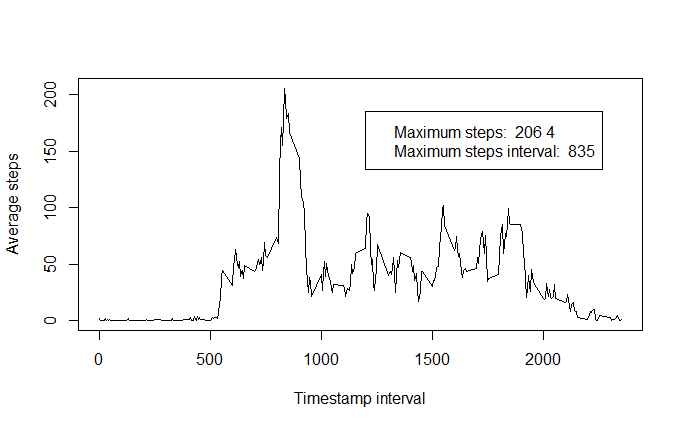
\includegraphics[width=1\linewidth]{./Rplot_2}

\hypertarget{imputing-missing-values}{%
\subsection{Imputing missing values}\label{imputing-missing-values}}

To answer this question, we need to do some calculations first.

\begin{enumerate}
\def\labelenumi{\arabic{enumi}.}
\tightlist
\item
  Calculating total amount of NA values:
\end{enumerate}

\begin{Shaded}
\begin{Highlighting}[]
\NormalTok{total_NA <-}\StringTok{ }\KeywordTok{as.integer}\NormalTok{(}\KeywordTok{nrow}\NormalTok{(activity_dt) }\OperatorTok{-}\StringTok{ }\KeywordTok{nrow}\NormalTok{(activity_dt_NM))}
\end{Highlighting}
\end{Shaded}

\begin{enumerate}
\def\labelenumi{\arabic{enumi}.}
\setcounter{enumi}{1}
\tightlist
\item
  Adding column to the data table with average steps values by interval:
\end{enumerate}

\begin{Shaded}
\begin{Highlighting}[]
\NormalTok{activity_dt_steps <-}\StringTok{ }\KeywordTok{merge}\NormalTok{(activity_dt, steps_ByInterval, }\DataTypeTok{by.x =} \StringTok{'interval'}\NormalTok{, }\DataTypeTok{by.y =} \StringTok{'Interval'}\NormalTok{)}
\end{Highlighting}
\end{Shaded}

\begin{enumerate}
\def\labelenumi{\arabic{enumi}.}
\setcounter{enumi}{2}
\tightlist
\item
  Filling NA values with average steps values:
\end{enumerate}

\begin{Shaded}
\begin{Highlighting}[]
\NormalTok{activity_dt_steps}\OperatorTok{$}\NormalTok{steps <-}\StringTok{ }\KeywordTok{ifelse}\NormalTok{(}\KeywordTok{is.na}\NormalTok{(activity_dt_steps}\OperatorTok{$}\NormalTok{steps), activity_dt_steps}\OperatorTok{$}\NormalTok{Avg_steps, }
\NormalTok{                                  activity_dt_steps}\OperatorTok{$}\NormalTok{steps)}
\end{Highlighting}
\end{Shaded}

\begin{enumerate}
\def\labelenumi{\arabic{enumi}.}
\setcounter{enumi}{3}
\tightlist
\item
  Calculating average steps by day:
\end{enumerate}

\begin{Shaded}
\begin{Highlighting}[]
\NormalTok{steps_ByDay2 <-}\StringTok{ }\KeywordTok{aggregate}\NormalTok{(activity_dt_steps}\OperatorTok{$}\NormalTok{steps, }\DataTypeTok{by =} \KeywordTok{list}\NormalTok{(activity_dt_steps}\OperatorTok{$}\NormalTok{date), sum)}
\KeywordTok{colnames}\NormalTok{(steps_ByDay2) <-}\StringTok{ }\KeywordTok{c}\NormalTok{(}\StringTok{'Days'}\NormalTok{, }\StringTok{'Total_steps'}\NormalTok{)}
\end{Highlighting}
\end{Shaded}

\begin{enumerate}
\def\labelenumi{\arabic{enumi}.}
\setcounter{enumi}{4}
\tightlist
\item
  Calculating the mean \& the median:
\end{enumerate}

\begin{Shaded}
\begin{Highlighting}[]
\NormalTok{steps_mean2 <-}\StringTok{ }\KeywordTok{round}\NormalTok{(}\KeywordTok{mean}\NormalTok{(steps_ByDay2}\OperatorTok{$}\NormalTok{Total_steps, }\DataTypeTok{na.rm =} \OtherTok{TRUE}\NormalTok{), }\DataTypeTok{digits =} \DecValTok{4}\NormalTok{) }
\NormalTok{steps_median2 <-}\StringTok{ }\KeywordTok{round}\NormalTok{(}\KeywordTok{median}\NormalTok{(steps_ByDay2}\OperatorTok{$}\NormalTok{Total_steps, }\DataTypeTok{na.rm =} \OtherTok{TRUE}\NormalTok{), }\DataTypeTok{digits =} \DecValTok{4}\NormalTok{)}
\end{Highlighting}
\end{Shaded}

\begin{enumerate}
\def\labelenumi{\arabic{enumi}.}
\setcounter{enumi}{5}
\tightlist
\item
  Final step, plotting the data along with the mean and the median:
\end{enumerate}

\begin{Shaded}
\begin{Highlighting}[]
\KeywordTok{ggplot}\NormalTok{(}\DataTypeTok{data =}\NormalTok{ steps_ByDay2, }\KeywordTok{aes}\NormalTok{(}\DataTypeTok{x=}\NormalTok{Days, }\DataTypeTok{y =}\NormalTok{ Total_steps)) }\OperatorTok{+}
\StringTok{              }\KeywordTok{geom_histogram}\NormalTok{(}\DataTypeTok{stat =} \StringTok{'identity'}\NormalTok{, }\KeywordTok{aes}\NormalTok{(}\DataTypeTok{fill =}\NormalTok{ Total_steps)) }\OperatorTok{+}
\StringTok{  }\CommentTok{#adding mean & median geoms}
\StringTok{              }\KeywordTok{geom_hline}\NormalTok{(}\KeywordTok{aes}\NormalTok{(}\DataTypeTok{yintercept =}\NormalTok{ steps_mean2, }\DataTypeTok{color =} \KeywordTok{paste}\NormalTok{(}\StringTok{'Mean: '}\NormalTok{, steps_mean2)), }
                         \DataTypeTok{linetype =} \DecValTok{2}\NormalTok{, }\DataTypeTok{size =} \DecValTok{1}\NormalTok{) }\OperatorTok{+}
\StringTok{              }\KeywordTok{geom_hline}\NormalTok{(}\KeywordTok{aes}\NormalTok{(}\DataTypeTok{yintercept =}\NormalTok{ steps_median2, }\DataTypeTok{color =} \KeywordTok{paste}\NormalTok{(}\StringTok{'Median: '}\NormalTok{, steps_median2)), }
                         \DataTypeTok{linetype =} \DecValTok{2}\NormalTok{, }\DataTypeTok{size =} \DecValTok{1}\NormalTok{) }\OperatorTok{+}
\StringTok{              }\KeywordTok{scale_color_manual}\NormalTok{(}\StringTok{'Mean & Median'}\NormalTok{, }\DataTypeTok{values =} \KeywordTok{c}\NormalTok{(}\DecValTok{1}\NormalTok{, }\DecValTok{2}\NormalTok{))}
\end{Highlighting}
\end{Shaded}

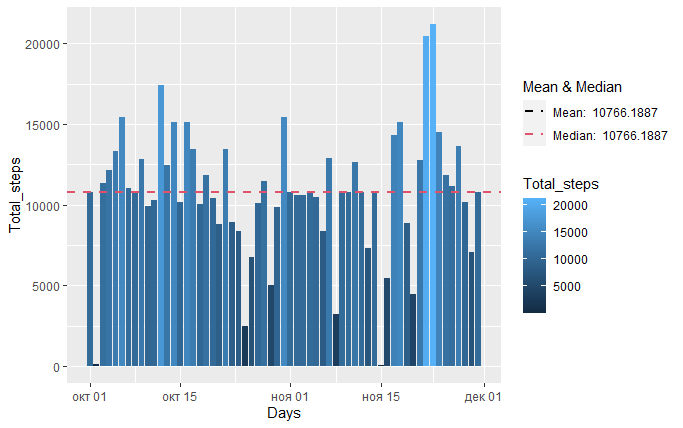
\includegraphics[width=1\linewidth]{./Rplot_3}

\hypertarget{are-there-differences-in-activity-patterns-between-weekdays-and-weekends}{%
\subsection{Are there differences in activity patterns between weekdays
and
weekends?}\label{are-there-differences-in-activity-patterns-between-weekdays-and-weekends}}

To answer this question, we need to do some calculations and
transformations first.

\begin{enumerate}
\def\labelenumi{\arabic{enumi}.}
\tightlist
\item
  Adding a column with weekdays to the data table:
\end{enumerate}

\begin{Shaded}
\begin{Highlighting}[]
\NormalTok{activity_dt_steps <-}\StringTok{ }\NormalTok{activity_dt_steps }\OperatorTok\StringTok{ }\KeywordTok{mutate}\NormalTok{(}\DataTypeTok{day =} \KeywordTok{weekdays}\NormalTok{(date))}
\end{Highlighting}
\end{Shaded}

\begin{enumerate}
\def\labelenumi{\arabic{enumi}.}
\setcounter{enumi}{1}
\tightlist
\item
  Custom function for checking whether a day is a weekday or a weekend
  day:
\end{enumerate}

\begin{Shaded}
\begin{Highlighting}[]
\NormalTok{check_day <-}\StringTok{ }\ControlFlowTok{function}\NormalTok{(day) \{}
  \KeywordTok{ifelse}\NormalTok{(day }\OperatorTok\StringTok{ }\KeywordTok{c}\NormalTok{(}\StringTok{'monday'}\NormalTok{, }\StringTok{'tuesday'}\NormalTok{, }\StringTok{'wednesday'}\NormalTok{, }\StringTok{'thursday'}\NormalTok{, }\StringTok{'friday'}\NormalTok{), }
         \KeywordTok{return}\NormalTok{(}\StringTok{'weekday'}\NormalTok{), }\KeywordTok{return}\NormalTok{(}\StringTok{'weekend'}\NormalTok{))}
\NormalTok{\}}
\end{Highlighting}
\end{Shaded}

\begin{enumerate}
\def\labelenumi{\arabic{enumi}.}
\setcounter{enumi}{2}
\tightlist
\item
  Adding a column with a day type to the data table:
\end{enumerate}

\begin{Shaded}
\begin{Highlighting}[]
\ControlFlowTok{for}\NormalTok{ (i }\ControlFlowTok{in} \DecValTok{1}\OperatorTok{:}\StringTok{ }\KeywordTok{nrow}\NormalTok{(activity_dt_steps)) \{}
\NormalTok{  activity_dt_steps}\OperatorTok{$}\NormalTok{dayType[i] <-}\StringTok{ }\KeywordTok{check_day}\NormalTok{(activity_dt_steps}\OperatorTok{$}\NormalTok{day[i])}
\NormalTok{\} }
\end{Highlighting}
\end{Shaded}

\begin{enumerate}
\def\labelenumi{\arabic{enumi}.}
\setcounter{enumi}{3}
\tightlist
\item
  Final step, plotting the data:
\end{enumerate}

\begin{Shaded}
\begin{Highlighting}[]
\NormalTok{steps_ByInterval_mean <-}\StringTok{ }\KeywordTok{aggregate}\NormalTok{(steps}\OperatorTok{~}\NormalTok{interval}\OperatorTok{+}\NormalTok{dayType, }\DataTypeTok{data=}\NormalTok{activity_dt_steps, mean)}
\KeywordTok{xyplot}\NormalTok{(steps}\OperatorTok{~}\NormalTok{interval}\OperatorTok{|}\KeywordTok{factor}\NormalTok{(dayType), }\DataTypeTok{data=}\NormalTok{steps_ByInterval_mean, }\DataTypeTok{aspect=}\DecValTok{1}\OperatorTok{/}\DecValTok{2}\NormalTok{, }\DataTypeTok{type=}\StringTok{"l"}\NormalTok{)}
\end{Highlighting}
\end{Shaded}

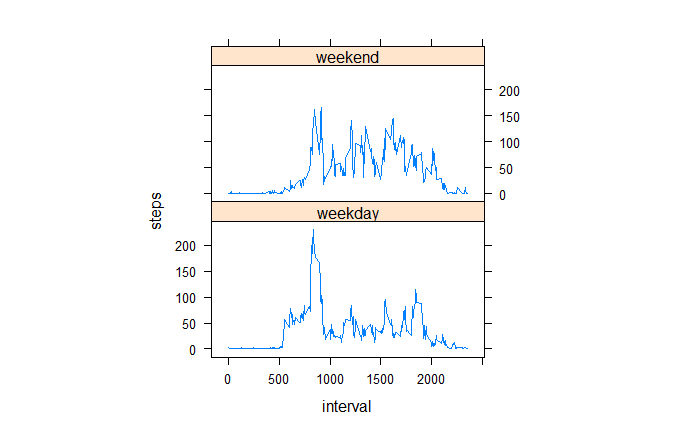
\includegraphics[width=1\linewidth]{./Rplot_4}

\end{document}
